\documentclass[
% opciók nélkül: egyoldalas nyomtatás, elektronikus verzió
% twoside,     % kétoldalas nyomtatás
% tocnopagenum,% oldalszámozás a tartalomjegyzék után kezdődik
]{thesis-ekf}
\usepackage[T1]{fontenc}
\PassOptionsToPackage{defaults=hu-min}{magyar.ldf}
\usepackage[magyar]{babel}

\usepackage{listings,lmodern,caption,mathtools,amssymb,amsthm,pdfpages}
\footnotestyle{rule=fourth}
\usepackage[usenames,dvipsnames]{xcolor}
\newtheorem{tetel}{Tétel}[chapter]
\theoremstyle{definition}
\newtheorem{definicio}[tetel]{Definíció}
\theoremstyle{remark}
\newtheorem{megjegyzes}[tetel]{Megjegyzés}

\definecolor{darkgreen}{rgb}{0, .7, 0}
\definecolor{lightorange}{rgb}{255, 165, 0}

\lstdefinestyle{php}{
	inputencoding=utf8/latin2,
	language=PHP,
	basicstyle=\footnotesize\ttfamily,
	columns=fullflexible,
	numbers=left,
	breaklines,
	xleftmargin=1cm,
	xrightmargin=1cm,
	postbreak=\hbox{$\color{red}\hookrightarrow$\ },
	backgroundcolor=\color{gray!30},
	frame=ltrb,
	keywordstyle=\bfseries\color{RoyalBlue},
	commentstyle=\itshape\color{teal},
	stringstyle=\bfseries\color{PineGreen},
	identifierstyle = \bfseries\color{YellowOrange},
	morekeywords=[1]{},
	keywordstyle=[3]{\bfseries\color{red}}
}
\renewcommand{\lstlistingname}{kódrészlet}

\begin{document}
\institute{Matematikai és Informatikai Intézet}
\title{Jelenlét és hiányzás követő alkalmazás fejlesztése}
\author{Györkis Tamás\\Programtervező informatikus BSc}
\supervisor{Dr. Király Roland\\Egyetemi docens}
\city{Eger}
\date{2024}
\maketitle
\tableofcontents

\chapter*{Bevezetés}
\addcontentsline{toc}{chapter}{Bevezetés}
Amikor szakdolgozati témaválasztás előtt álltam, sokat gondolkoztam a témán. Mindenképpen egy olyan alkalmazást szerettem volna elkészíteni, mely ténylegesen hasznos is lehet. Egyetemi éveim alatt demonstrátorként tanítottam több féléven át az egyetemen, és innen jött a felismerés, hogy jó lenne, ha a hallgatók jelenlétét, hiányzásait ne táblázatokban kelljen vezetni, hanem egy külön eszköz legyen rá készítve. Innen származik az alkalmazás ötlete.

A megvalósítás során törekedtem arra, hogy egy jól átlátható, ergonomikus weboldalt készítsek, amit -- esetleges kisebb módosításokkal -- ne csak egyetemi környezetben lehessen használni. Ezekből kifolyólag egy webalkalmazást készítettem, mivel ezt a legegyszerűbb elérni, hiszen csak egy webböngésző szükséges hozzá. A tanulók és tanárok által használt oldalak reszponzívan lettek elkészítve, ezáltal biztosítva, hogy mobiltelefonon is használni lehessen. Illetve az alkalmazás PWA\footnote{Jelentése: Progressive Web App: egy olyan alkalmazás, ami webes technológiákat használ, de platform specifikus alkalmazásként viselkedik.\cite{PWA}}  funkciókkal rendelkezik, aminek jelentőségére később térek ki, de előjáróban annyit érdemes megemlíteni róla, hogy lehetővé teszi a weboldal alkalmazásként való telepítését számítógép és telefon esetén is, ezáltal egy rendes alkalmazás érzését keltve.

A megvalósításhoz a Laravel keretrendszert használtam, mely egy PHP alapú, MVC\footnote{Jelentése: Model-View-Controller.\cite{mvc}} keretrendszer, amivel tanulmányaim során találkoztam, és egyből megkedveltem. Nem titkolt célom a szakdolgozatommal, hogy bemutassam, hogy a mai, JavaScript preferált világban, továbbra is lehetséges modern, a mai kort kielégítő weboldalt készíteni PHP segítségével, amihez különböző csomagokat alkalmaztam, amiknek működését, illetve egymással való működését a későbbiekben fogom kifejteni.

Szakdolgozatom négy részre osztottam: \aref{appDescription}. fejezetben magát az alkalmazást mutatom be. \Aref{packages}. fejezetben magát a keretrendszert, illetve a használt csomagokat, ezek hogy működnek együtt. Végül \aref{testing}. és \aref{setup}. fejezetben a tesztelést és a telepítést részletezem.

\chapter{Alkalmazás bemutatása}
\label{appDescription}
\section{Adatbázis}

\Aref{database} ábrán látható az alkalmazás által használt adatbázis, egyed-kapcsolat diagrammal ábrázolva, melyről szeretnék néhány szót ejteni.

\begin{figure}[ht!]
	\centering
	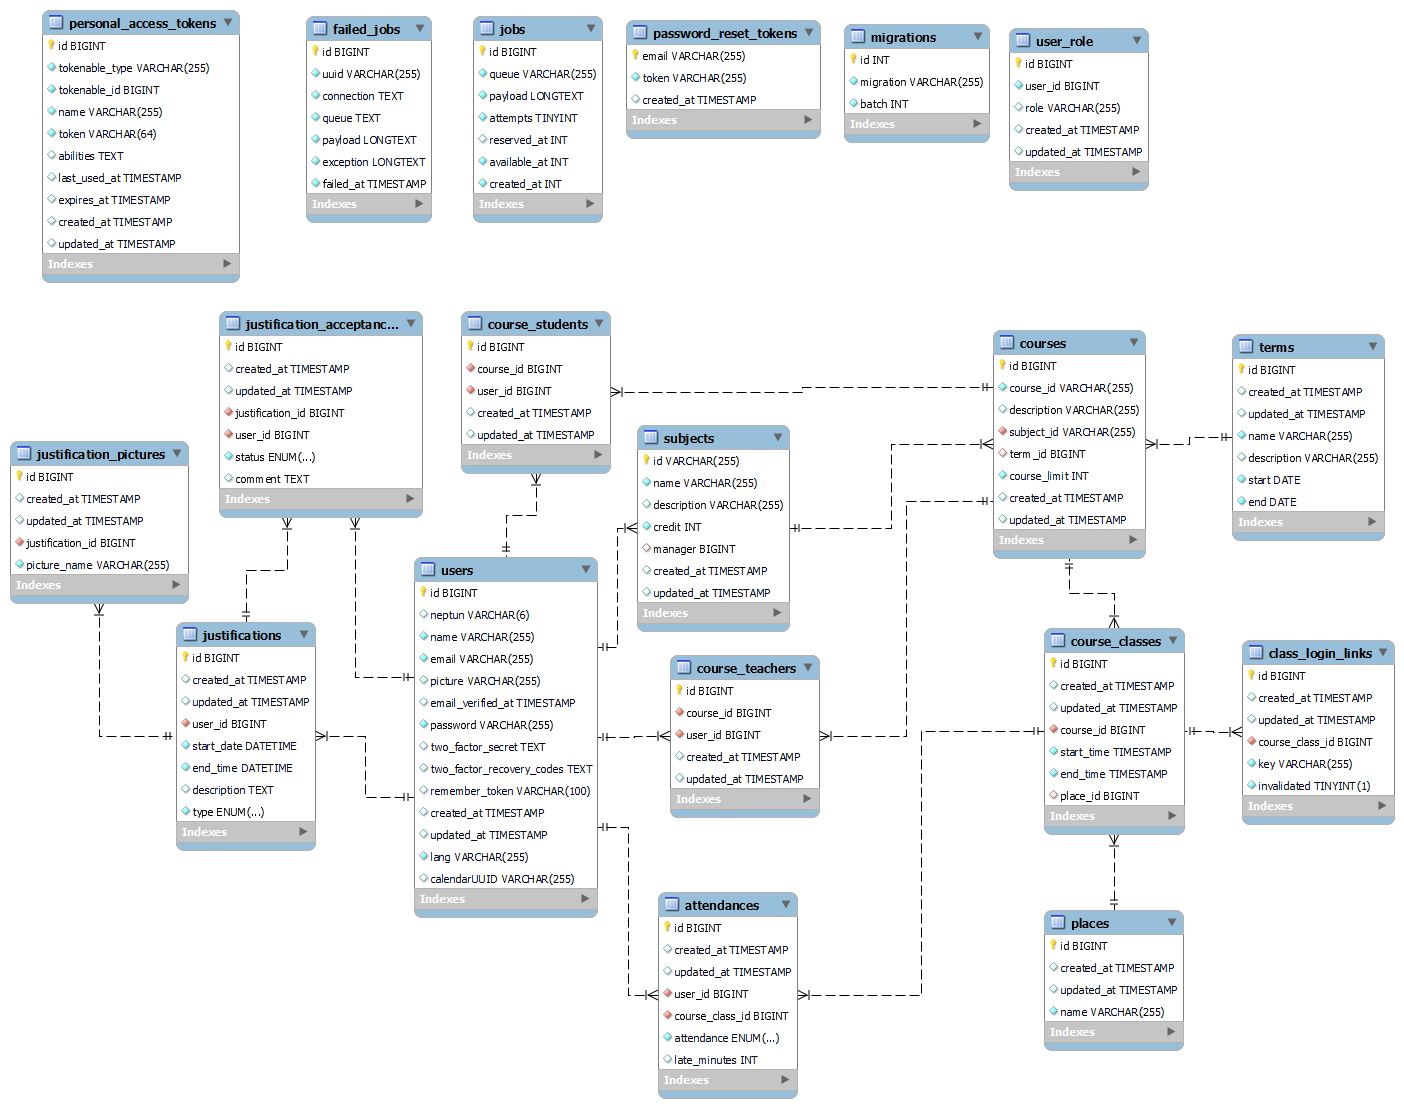
\includegraphics[width=15cm]{../pictures/db.png}
	\caption{Az alkalmazás által használt adatbázis.}
	\label{database}
\end{figure}

\begin{itemize}
	\item \emph{users, user\_roles}: ez a tábla tárolja a felhasználók adatait, illetve a felhasználókhoz tartozó jogosultsági köröket. Minden felhasználóról tárolunk egy azonosítót, egy Neptun\cite{Neptun} kódot\footnote{A neptun kód egy 6 karakter hosszú, egyedi azonosító.}, nevet, email címet, egy titkosított jelszót, egy profilképet, a felhasználó által használt nyelvet, illetve egy UUID-t\footnote{}, azaz egy egyedi azonosítót, amit az órarend exportálásához lehet használni, erről később. Az azonosító oszlopra azért van szükség, mivel az alkalmazás fel van készítve arra, hogy Neptun kód nélkül rendelkező felhasználókat is tudjon kezelni.
	\item \emph{terms, places}: a félévek és termek (helyek) tárolására szolgáló táblák.
	\item \emph{subjects, courses, course\_classe, class\_login\_links}: ezen táblák tárolják a tantárgyakat (amik többek között rendelkeznek egy azonosítóval, névvel, leírással, kreditértékkel, és egy tantárgyfelelőssel), a tantárgyakhoz tartozó kurzusokat (amihez tárolok egy azonosítót, ami minden esetben egyedi, egy kurzus azonosítót, ami minden félév és tantárgy esetében kell egyedinek lennie, tartozik hozzá egy félév, illetve egy létszám limit), illetve kurzusokhoz pedig órák (amiknek van egy kezdete, vége, illetve egy terem, ahol tartják). Az utolsó tábla pedig az órákhoz tartozó bejelentkező linkeket tartalmazza, ennek jelentőségéről kicsit később.
	\item  \emph{attendances}: itt tárolom az egyes kurzusok résztvevőinek az órai jelenléteit, melyek lehetnek: nincs kitöltve, jelen, késés (mely esetben percben lehet tárolni a mértékét), hiányzás, igazolt hiányzás.
	\item \emph{justification, justification\_acceptances, justification\_pictures}: ezek a táblák tárolják az igazolásokat, az igazoláshoz tartozó feltöltött képeket, illetve az igazolásban érintett tanárok válaszát, hogy elfogadják-e ó, vagy sem.
	\item Az egyéb, nem említett táblák inkább kapcsolótábla funkciót töltenek be, vagy a keretrendszernek vannak rá szükségei. Például a \emph{jobs} tábla a háttérben végrehajtandó feladatokat (job) tartalmazza.
\end{itemize}

Itt érdemes még megemlíteni, hogy a fejlesztés során a MySQL nevezetű, relációs adatbázist használtam, viszont a Laravel keretrendszerből adódóan sok más típusú adatbázis szoftverrel használható az alkalmazás, mivel a táblák felépítése a keretrendszer nyújtotta módon van elkészítve.

\section{Általános információk}

\subsection{Felhasználók}

Az alkalmazás 4 különböző jogkört különböztet meg a felhasználók esetén, melyekből egyszerre többet is birtokolhat a felhasználó:

\begin{itemize}
	\item Szuper adminisztrátor: képes a felhasználók adatainak -- és jogköreinek -- szerkesztésére, illetve az alkalmazás alapbeállításainak módosítására.
	\item Adminisztrátor: a félévek, termek, tantárgyak, kurzusok, órák, készítésére, módosítására, törlésére jogosult.
	\item Tanár: megtekintheti a tanított óráit, kurzusait, hallgatóit. Adminisztrálni tudja az órákon való részvételt, illetve megtekintheti és bírálhatja a hozzá érkezett igazolásokat.
	\item Hallgató: a hozzárendelt óráit, tantárgyait látja, megtekintheti minden kurzus esetén az egyes órák státuszát, illetve igazolásokat hozhat létre
\end{itemize}

Az alkalmazás természetesen rendelkezik bejelentkezés, regisztráció funkciókkal. A felhasználók Neptun\cite{Neptun} kódjuk vagy email címük, illetve a jelszavuk megadásával tudnak bejelentkezni. Regisztrálni csak abban az esetben tudnak, ha az oldal beállításaiban ezt engedélyezték, egyéb esetben a szuper adminisztrátorok tudnak felhasználókat létrehozni vagy importálni. Belépés után  a profil szerkeszthető, a jelszó cserélhető.

\subsection{Általános funkciók}

Bejelentkezés után a főoldalon a felhasználók pár, számukra fontos vagy érdekes információt láthatnak. Tanulók esetében a mai napi óráikat, illetve adminisztrálásra váró igazolásaikat. Tanárok esetén szintén a mai óráikat, illetve a kapott igazolásaikat láthatják. Az adminisztrátorok pár statisztikát láthatnak az oldal kapcsán.

\begin{figure}[ht!]
	\centering
	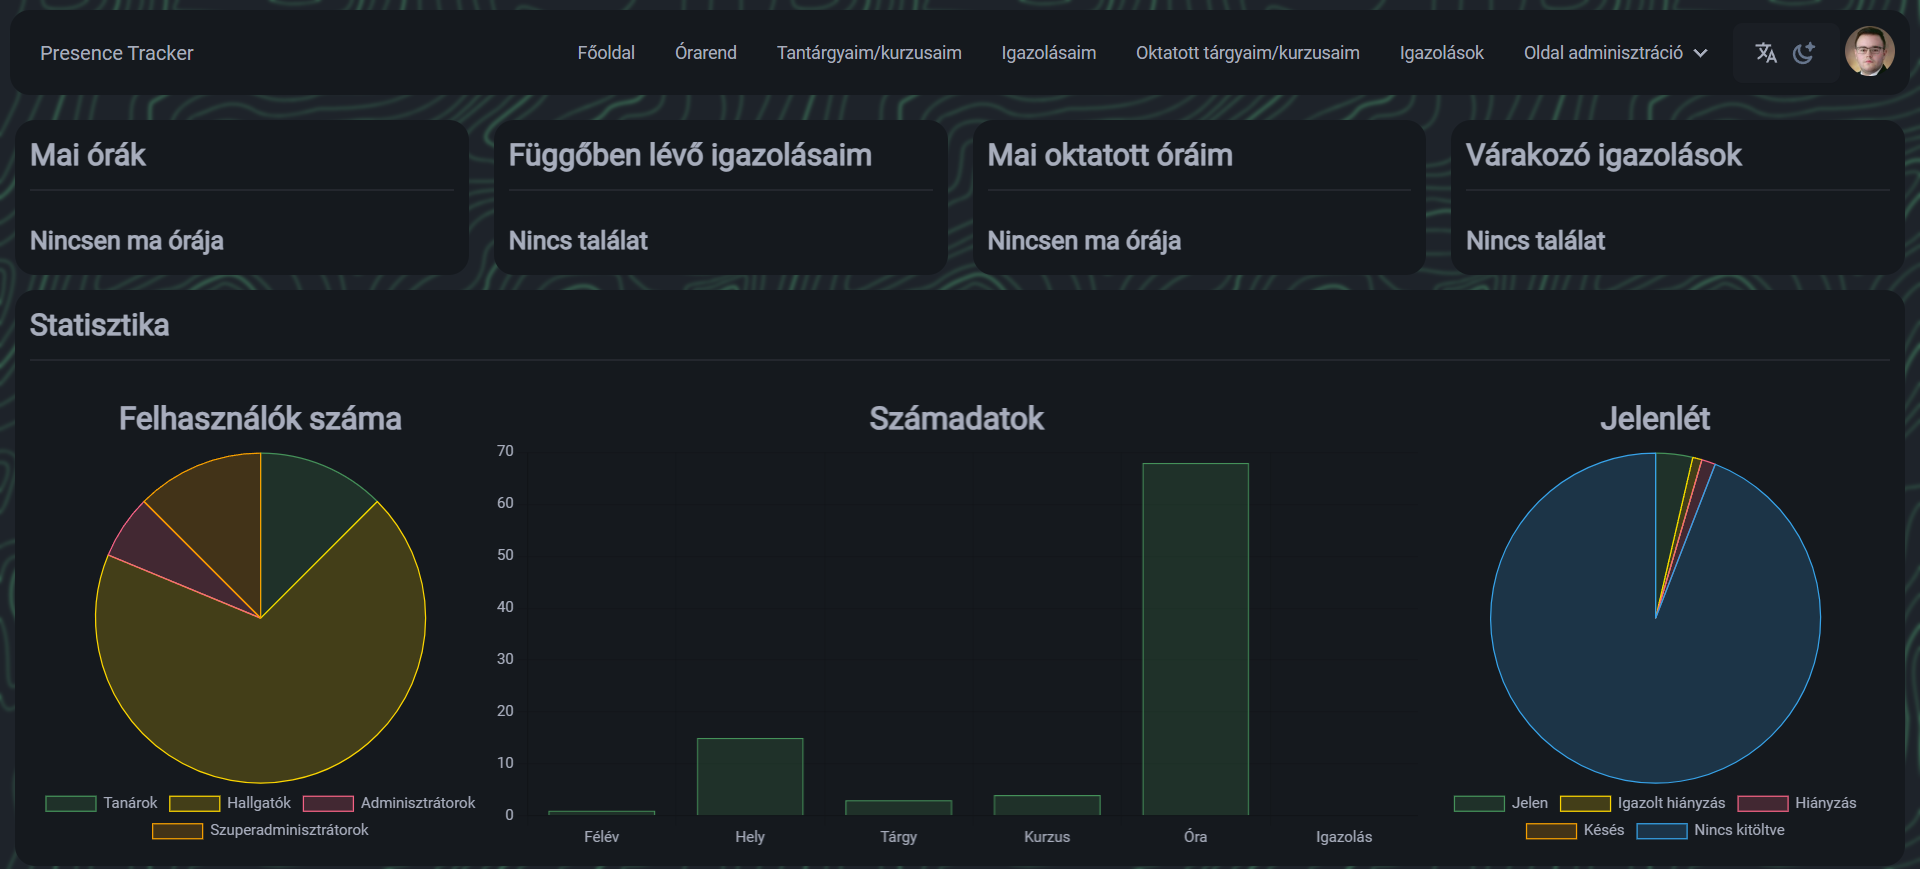
\includegraphics[width=10cm]{../pictures/screenshots/landing.png}
	\caption{A főoldal kinézete abban az esetben, ha a felhasználó minden szerepkörrel rendelkezik. A két bal oldali oszlop a hallgatói nézethez tartozik, a két jobb oldali pedig az oktatóihoz, míg a statisztika adminisztrátorok esetén jelenik meg.}
	\label{landing}
\end{figure}

A profil kép melletti gombra kattintva a felhasználó meg tudja változtatni az oldal nyelvét, Angol és Magyar nyelv közül választva, illetve az oldalt kinézetét: világos és sötét mód között váltogatva. A nyelv beállítása eltárolódik a felhasználóhoz, így újabb bejelentkezés esetén automatikusan beállításra kerül.

Tanuló vagy tanár esetén megjelenik az \emph{Órarend} menüpont is, ahol egy helyen láthatják a heti óráikat a felhasználók. Az egyes órák különböző színekkel jelennek meg, ezzel jelezve, hogy az adott órát a felhasználó tanítja-e, vagy hallgató esetén az órán jelen volt, hiányzott, késett, igazoltan hiányzott, vagy még nincs kitöltve a jelenlét. Lehetőség van az órarend exportálásra is, mely során egy \emph{.ics} kiterjesztésű fájl áll elő. Ez egy széles körben használt általános naptár formátum, amit a felhasználók be tudnak importálni a gyakorian használt naptár programokba\cite{ICS}. Ezáltal kedvenc naptár alkalmazásukban is nyomon tudják követni óráikat.

Lehetőség van a weboldalt alkalmazásként telepíteni, ahogy az \aref{install} ábrán is látható, így gyorsan hozzáférhetnek az alkalmazás funkcióihoz, egy ,,rendes'' alkalmazás érzését keltve ezzel. Ezt a PWA\footnote{Jelentése: Progressive Web App: egy olyan alkalmazás, ami webes technológiákat használ, de platform specifikus alkalmazásként viselkedik.\cite{PWA}} teszi lehetővé, melynek működésére későbbiekben térek ki.

\begin{figure}[ht!]
	\centering
	
\includegraphics[width=8cm]{../pictures/screenshots/install.png}
	\caption{Az oldal telepítésére szolgáló felugró ablak.}
	\label{install}
\end{figure}

\section{Adminisztrátori nézet, funkciók}

\subsection{Felhasználók kezelése}

Szuper adminisztrátor esetén a felhasználó képes kezelni az alkalmazásban tárolt felhasználókat, kivéve saját magát (személyes adatait továbbra is meg tudja változtatni). A listában képes szűrni a felhasználók között, megváltoztatni profil adataikat, jelszavukat alaphelyzetbe állítani, szerkeszteni jogosultsági szintjeiket, illetve akár törölni is őket, ha szükséges. Tud új felhasználókat létrehozni, illetve képes fájlból is importálni adatokat.

\subsection{Alkalmazás konfiguráció}

Szintén a szuper adminisztrátor körébe tartozik az oldal beállításainak kezelése. Az alábbi beállításokat tudja kezelni:
\begin{itemize}
	\item Oldal neve: az oldalon megjelenő név megváltoztatása.
	\item Regisztráció engedélyezése: ezzel lehet engedélyezni, hogy a felhasználók maguktól is tudjanak-e felhasználói fiókot készíteni az oldalon.
	\item Saját Neptun\cite{Neptun} kód megváltoztatása: beállítható, hogy a felhasználó meg tudja magának változtatni ezt az értéket, vagy sem.
	\item Kötelező Neptun kód: az oldal használható ezen kód megadása nélkül is, ez itt szabályozható.
	\item Alkalmazás képe: itt tölthető fel új kép, ami a fő oldalon jelenik meg látogatók esetén.
\end{itemize}

\subsection{Félévek, termek, tantárgyak, kurzusok, órák kezelése}

Minden adminisztrátor képes ezen adatok kezelésére.

Félévek esetén egy nevet, illetve egy kezdő és vég dátumot szükséges megadni. Ellenőrizve van, hogy a félévek nem ütközhetnek egymással. A listában egy pipa jelzi a jelenlegi félévet, ha van ilyen.

A termeknél elegendő egy nevet megadni, ezeket lehet az egyes órákhoz hozzárendelni.

Tantárgyak esetén egy tárgy kódot, egy nevet, egy opcionális leírást, egy kredit értékéket, illetve egy tantárgyfelelőst tárol, akinek rálátása van a tárgy összes kurzusára. Ezen belül minden kurzus egy tárgyhoz kapcsolódik. Ezek szintén rendelkeznek egy kóddal, ami minden tárgy és félév esetén egyedi, szintén egy opcionális leírással, illetve nulla, egy, vagy több tanárral. Minden kurzus egy félévhez van rendelve. A kurzusokhoz hozzárendelhetők a hallgatók, és csak hallgatók.

A kurzusokhoz órák hozhatóak létre, amik a féléven belül lehetnek. Minden óra külön kezdés és vég időponttal rendelkezik, illetve egy teremmel, ahol tartják. Az óra létrehozásakor lehetőség van arra is, hogy a félév végig heti ismétléssel hozza létre az órákat -- természetesen később egyenként lehet őket szerkeszteni, törölni --, ezáltal megkönnyítve az adminisztrációt.

\begin{figure}[ht!]
	\centering
	
\includegraphics[width=15cm]{../pictures/screenshots/newclass.png}
	\caption{Új óra hozzáadása.}
	\label{newclass}
\end{figure}


\section{Tanári nézet, funkciók}

\subsection{Oktatott tárgyak}

A tanárok megtekinthetik az általuk oktatott -- vagy tantárgyfelelősként hozzáadott -- tárgyakat, és az azokhoz kapcsolódó adatokat. Igény szerint szűrhetnek kód, név, vagy félévre is. Minden kurzus esetén megtekinthetik az alap adatokat, a kurzushoz tartozó órákat, hallgatókat. Itt van lehetősége a tanárnak hozzáadni hallgatókat a kurzushoz, illetve egy listában megtekinteni diákokra lebontva, hogy mennyit hiányoztak, mennyit késtek, ebből mennyi az igazolatlan.

A kurzus órái listában érhetik el az egyes órákat, ahol adminisztrálhatják a jelenlétet. Egy órát megnyitva láthatják az ahhoz kapcsolódó adatok, illetve bal oldalon egy listát a kurzus tanulóiról, ahol beállíthatják a hallgató státuszát. Amennyiben az adott hallgató a tanár által elfogadott igazolással rendelkezik, akkor ebben az esetben csak ,,jelen'' státusz -- ha esetleg mégis megjelent az órán --, vagy pedig ,,igazol hiányzás'' státusz állítható be, illetve egy figyelmeztető üzenet is megjelenik. Ezek mellett megjelenik az adott kurzuson való összes hiányzás és igazolt hiányzások száma is. Hiányzás rögzítése esetén email üzenet formájában is értesítést kap a hallgató.

A jobb oldalt kettő doboz foglal helyet. Az első egy Qr\footnote{A Qr kód egy információt tartalmazó kép,  amit kamerával lehet leolvasni.\cite{QR}} kódot tartalmaz. Ennek segítségével, ha az oktató látható teszi, a diákok a kódot a telefonjukon beolvasva, majd bejelentkezve is ,,beírhatják magukat'' az órára, ezzel felgyorsítva a folyamatot, és a tanárnak sem kell végig mennie a listán. A kód csak az óra végéig működik, illetve ha az oktató úgy sejti, hogy a hallgatók visszaélnek ezzel, akkor hamarabb is letilthatja, illetve generálhat egy másikat. Amikor a hallgató íj módon bejelentkezik az órára, a tanári felületen automatikusan frissítésre kerül a státusz. A hallgató csak abban az esetben tudja ezt a funkciót használni, hogy ha fel van iratkozva a kurzusra, és még nem állították be az adott órára a státuszát, ezzel elkerülve, hogy magától átírja esetleges hiányzását, késését.

A másik ilyen doboz egy kis statisztikát mutat kör diagram formájában, megszámolva a hallgatók státuszát az órán.

\begin{figure}[ht!]
	\centering
	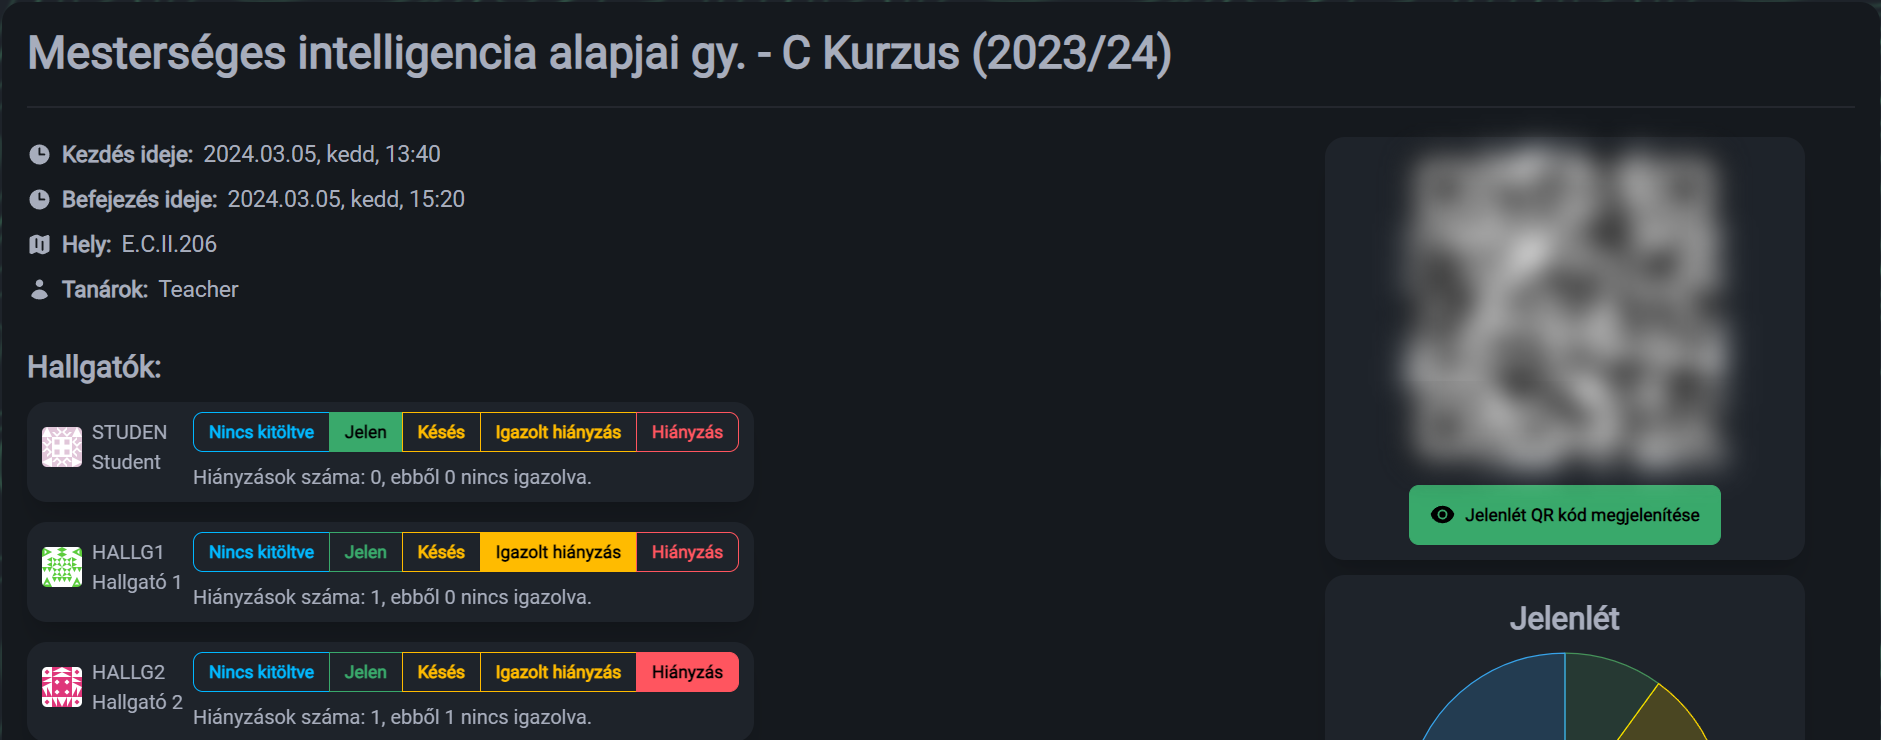
\includegraphics[width=10cm]{../pictures/screenshots/class_1.png}
	\caption{Egy óra nézete.}
	\label{class}
\end{figure}

\begin{figure}[ht!]
	\centering
	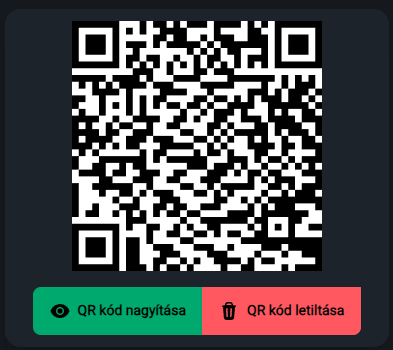
\includegraphics[width=6cm]{../pictures/screenshots/class_2.png}
	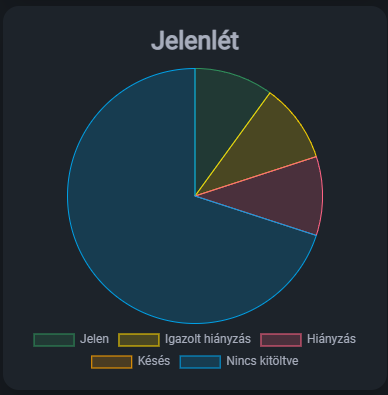
\includegraphics[width=6cm]{../pictures/screenshots/class_3.png}
	\caption{Egy óra kártyái.}
	\label{class2}
\end{figure}

\subsection{Igazolások}

Amikor egy hallgató igazolást ad le, akkor azt minden érintett tanár megkapja, és reagálhat rá; vagy elfogadja, vagy indoklással elutasítja. A lista alapból szűrésre kerül, hogy csak a még nem meg válaszolt igazolásokat mutassa az oktatónak. Amikor a tanár megnyit egy ilyen igazolást, láthatja, hogy ki küldte be az igazolást, a típusát (orvosi vagy egyéb), az kezdeti és vég időpontot, illetve az esetlegesen feltöltött képeket is megtekintheti. Ezek mellett listába szedve, és tantárgy, majd kurzus alapján kategorizálva látja az általa oktatott és az igazolásban érintett órákat, azok idejét, illetve a hallgató jelenlegi státuszát az órán. Az igazolás elfogadása esetén azon órák, ahol nem ,,jelen''-re van állítva az állapot, automatikusan ,,igazolt hiányzás'' állapotra kerülnek beállításra. Elfogadás és elutasítás esetén is üzenet kap a hallgató, illetve a főoldalon megtekintheti a még függőben lévő (tehát nem minden érintett tanár által megválaszolt) igazolásait is.

\begin{figure}[ht!]
	\centering
	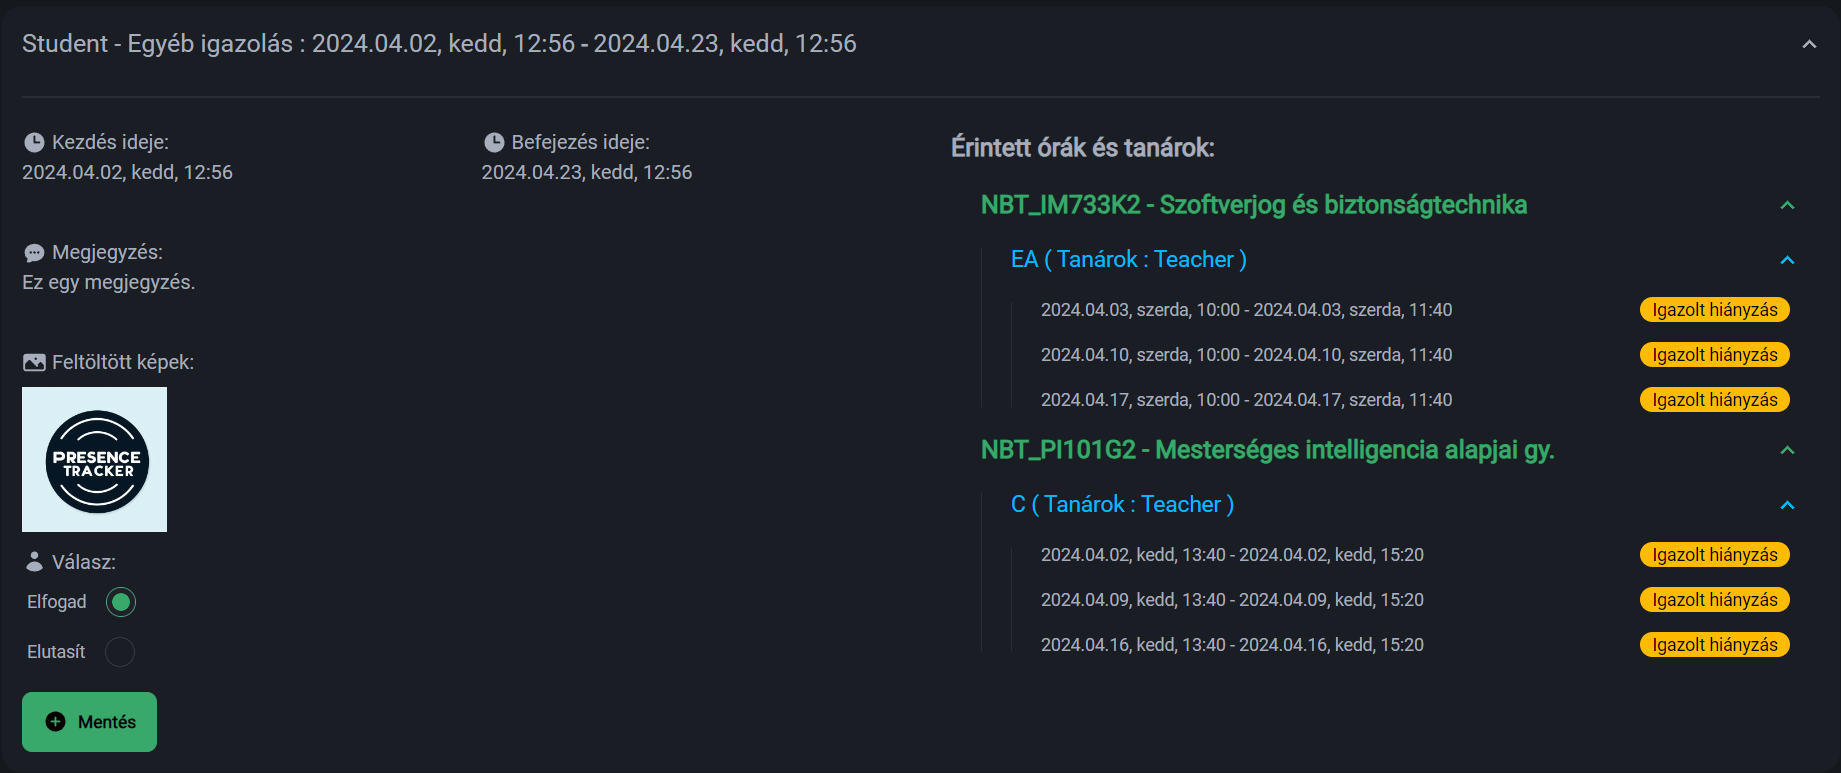
\includegraphics[width=15cm]{../pictures/screenshots/just_teacher.png}
	\caption{Egy elfogadott igazolás, ahogy a tanár látja.}
	\label{justTeacher}
\end{figure}

\section{Hallgatói nézet, funkciók}

\subsection{Tantárgyak, kurzusok}

A hallgatók természetesen láthatják a tantárgyaikat, amiket csakugyan szűrhetnek név, kód, félév szerint. Itt egy helyen megtekinthetik kurzusokra lebontva, hogy melyik órán milyen státusz van rögzítve, illetve egy diagramon ezeknek az eloszlását. Megtekinthetik még a kurzuson lévő hallgatótársaikat is.

\begin{figure}[ht!]
	\centering
	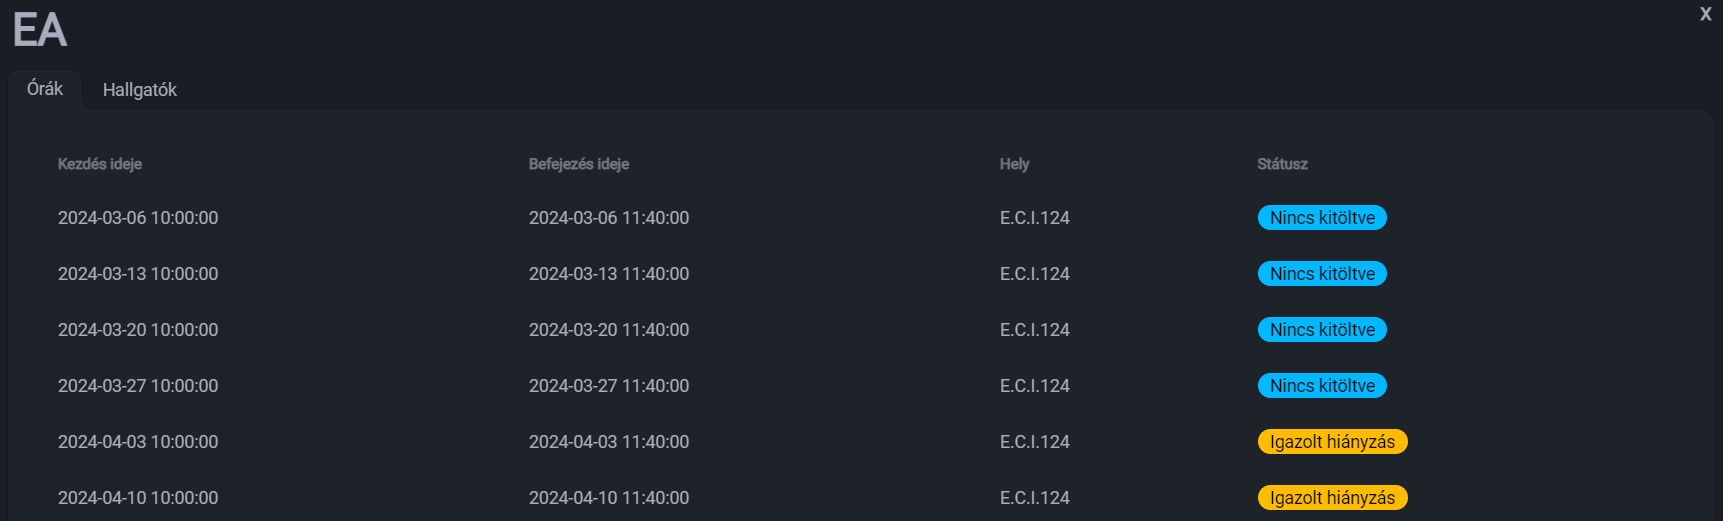
\includegraphics[width=12cm]{../pictures/screenshots/student_course.png}
	\caption{A hallgató által látott egy kurzus részlete.}
	\label{studentCourse}
\end{figure}

\subsection{Hallgató által létrehozott igazolások}

A hallgató a hiányzásainak igazolására igazolásokat adhat le a rendszerben. A létrehozáskor meg kell adnia a típusát (orvosi vagy egyéb), a kezdeti és vég dátumát, illetve szükség szerint megjegyzést fűzhet, illetve képeket tölthet fel, például az orvosi igazolást lefényképezheti. A dátumok megadása után a hallgató is látja az érintett óráit listába szedve.

Helyes adatok megadása és mentés után a listában is megjelenik az igazolás, amit lenyitva látja a megadott részelteket, illetve az egyes tanárok visszajelzését is, hogy elfogadták-e vagy sem. Amennyiben úgy látja, hogy elrontott valamit, akkor itt törölheti az igazolást, és hozhatja újra létre.

\begin{figure}[ht!]
	\centering
	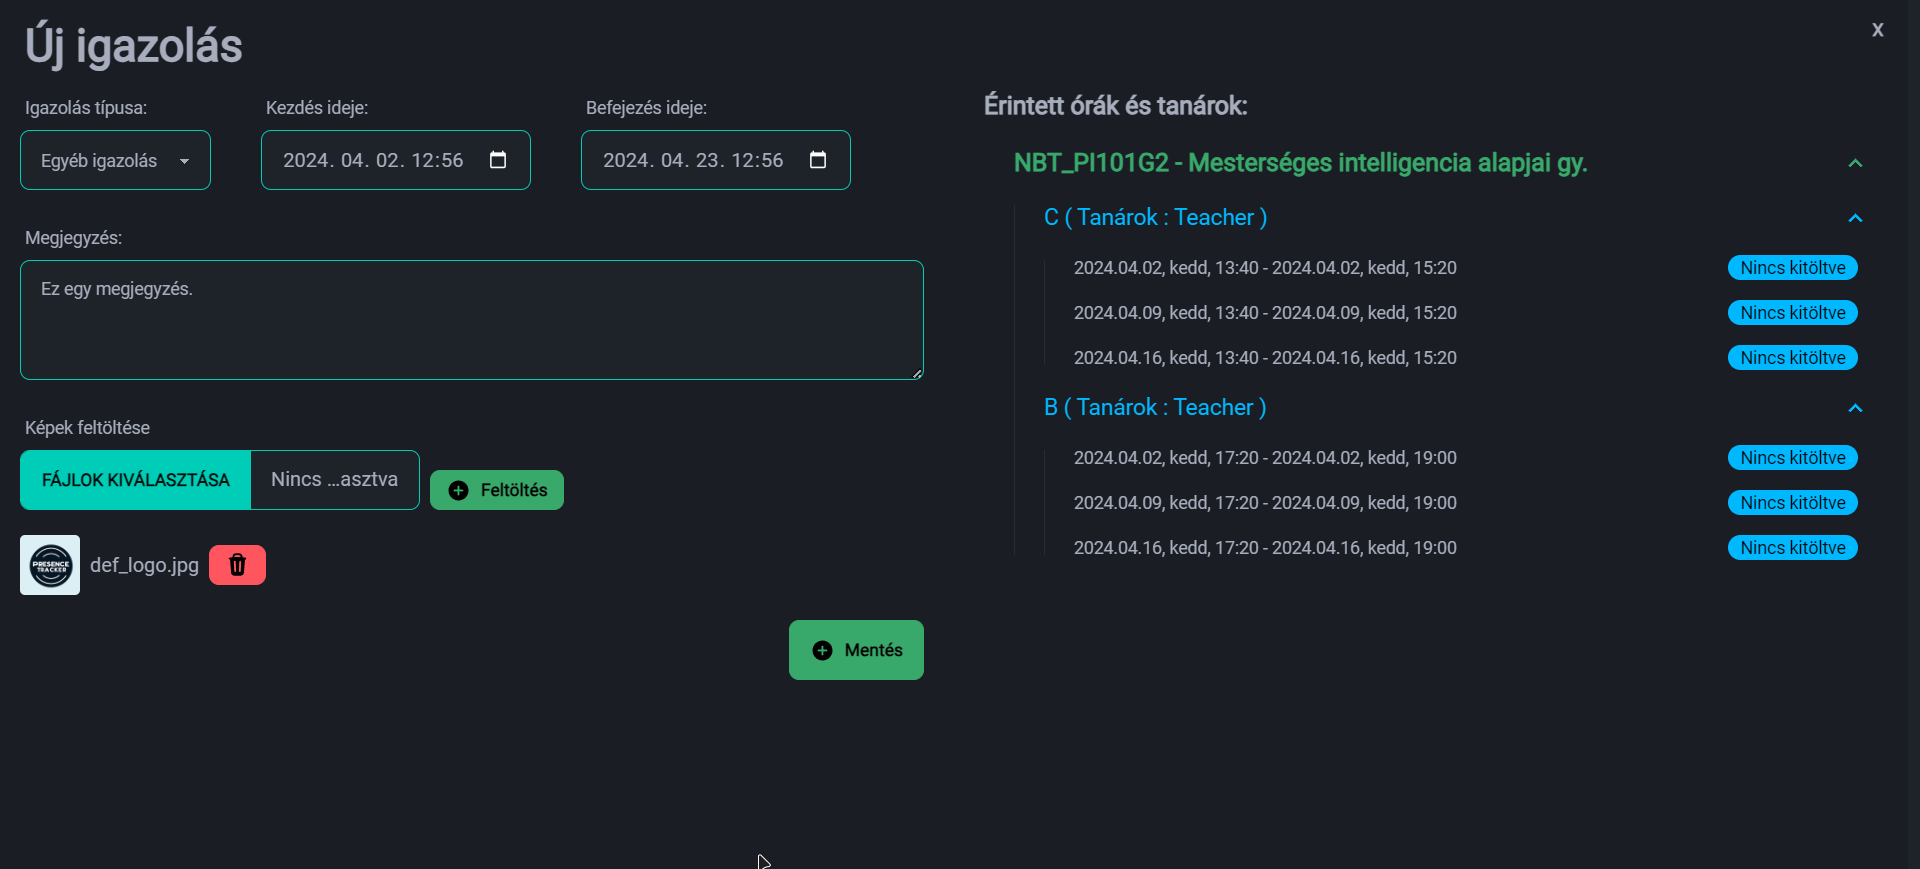
\includegraphics[width=12cm]{../pictures/screenshots/newJust.png}
	\caption{A hallgató által látott egy kurzus részlete.}
	\label{studentJustification}
\end{figure}

\chapter{Felhasznált technológiák, csomagok}
\label{packages}
\section{Laravel}

Ahogy a bevezetőben említettem, a megvalósításhoz a Laravel nevezetű keretrendszert használtam. A keretrendszer sok funkciót alapból elkészít, amit hosszadalmas lenne újra és újra megírni, ezáltal a programozó a lényegre fókuszálhat: az elkészítendő programra.\cite{meetlaravel}

\subsection{Keretrendszer alapjai}

\subsubsection{MVC architektúra}

A keretrendszer az MVC architektúrát követi, ami segíti a kód karbantartását, áttekinthetőségét.\cite{mvc} Ez azt jelenti, hogy logikailag a kód három része bomlik:
\begin{itemize}
	\item Modellek (Model): ezek tartalmazzák az adatbázis táblák modelljeit, ezeken keresztül tudjuk elérni az adatbázisunkat, illetve az adatbázisban tárolt adatokat is modellek formájában kapjuk meg, így ezeknek követni kell a táblák felépítését. Ezek mellett kapcsolatokat is meg tudunk adni a modellek között.
	\item Nézet (View): itt magára a nézetekre kell gondolni, amit látni fog a felhasználó. Ezek jelen esetben a Blade\cite{blade} fájlok, amire \aref{bladeSection}. alfejezetben térek ki.
	\item Kontroller (Controller): az üzleti logikát tartalmazza. Itt kapnak helyet a függvények például, amik egy kérés fogadásakor futnak le.
\end{itemize}

\subsubsection{Útvonalak}

A keretrendszerben az útvonalakat a \emph{routes} mappában található fájlokban találjuk. Mivel a keretrendszer képes nem csak webes kéréseket kiszolgálni, így több fájlra vannak szedve, viszont én csak a webes útvonalakhoz tartozó fájlt használtam.

Útvonalakat a \emph{Route} osztály metódusaival tudunk létrehozni. Ezek után meg kell adnunk a útvonal típusát (tehát hogy \emph{Get, Post, Put vagy Delete} típusú útvonalat szeretnénk létrehozni), magát az elérési útvonalat, illetve a meghívandó programkódot, ami ki fogja szolgálni a kérést. Opcionálisan megadhatunk egy nevet is, amivel referálni tudunk rá a kódunk többi részéből, illetve adhatunk meg egy vagy több köztes program kódot (angolul: middleware), mellyel kontrollálhatjuk az útvonal elérést és egyéb más dolgokat tehetünk meg a kérés kiszolgálása előtt.\cite{routing} Erre láthatunk egy példát \aref{routesandMiddleware} kódban.

Amennyiben az olvasó megnézi az elkészült programban található útvonalakat, azt láthatja, hogy csak \emph{Get} típusú útvonalak találhatóak benne. Ennek fő oka a Livewire\cite{livewire} használata, ahol útvonalak létrehozása helyett metódushívásokkal történik sok interakció, erről \aref{livewireSection}. alfejezetben lesz szó.

\subsubsection{Middleware}

A middleware arra alkalmas, hogy a kérés feldolgozása előtt végezzünk el teendőket, akár szűrjük őket.\cite{middleware} A program során én három fő dologra használtam ezt fel: bejelentkezés vizsgálata, hozzáférési jogosultság vizsgálata, illetve a kérés elején az alkalmazás nyelvének beállítása. Az utolsóra azért volt szükség, mivel Laravel esetén a nyelv beállítása mindig csak az adott kérésre vonatkozik. Így minden esetben meg kellett vizsgálni, hogy a felhasználó átállította-e a nyelvet, és ha igen, akkor alkalmazzuk a kiválasztott nyelvet a kérésre. A middleware futása során dönthetünk úgy is, hogy a kérést megszakítjuk, például ha a felhasználó nem rendelkezik kellő jogosultsággal. Hozzá is tudjuk rendelni ezeket az egyes útvonalakhoz, ahogy az \aref{routesandMiddleware}. kódrészleten látható, vagy akár beállíthatjuk, hogy globálisan, minden kérés esetén lefusson az adott kód.

\lstinputlisting[caption={Egy \emph{Get} típusú útvonal, ami az órarendet nyitja meg. Az útvonal meghívásakor a \emph{Controller} nevű osztály \emph{getTimetable} metódusa fut le. Az útvonalat csak bejelentkezett felhasználók ('auth') és diákok vagy tanárok ('studentorteacher') érhetik el.}, label=routesandMiddleware, style=php]{../codes/route.php}

\subsubsection{Konfiguráció}

A \emph{config} mappában találhatók a konfigurációs. Ha jobban megnézzük, ezek igazából PHP fájlok, amik egy tömb-ként adják vissza a konfigurációs értékeket. Ezeket módosíthatjuk, illetve mi is hozhatunk újakat létre. Én is így tettem: az olyan beállításokat, mint például, hogy engedélyezve van-e a regisztráció, vagy hogy a felhasználók módosíthatják-e a kódjukat, innen kérdezem le. Sok esetben az értékeket a környezeti konfigurációs fájlból olvassa be a program, ezáltal a gyakran változó értékek egy helyen módosíthatók anélkül, hogy keresni kéne őket, hogy hol vannak.

\subsubsection{Nyelvesítés}

\subsection{Eloquent ORM}
\subsection{Blade templating engine}
\label{bladeSection}
\subsection{Laravel Fortify}
\subsection{Jogosultság kezelés}
\subsection{Események, queue}
\subsection{Email küldés}

\section{Tailwind}
\subsection{DaisyUI}

\section{LiveWire}
\label{livewireSection}
\subsection{Ismertető, a csomag működése}
\subsection{LiveWire és SPA}
\subsection{Komponensek és data binding}
\subsection{Események, lapozás}
\subsection{Alpine.js: LiveWire és JavaScript kapcsolata}
\subsection{WireToast: LiveWire alapú értesítések}

\section{Websocket és Pusher szerviz}
\subsection{Websocket jelentősége}
\subsection{Pusher}
\subsection{Websocket integrálása a keretrendszerbe}
\subsection{Csatornák, események létrehozása}
\subsection{Események fogadása JavaScript, LiveWire esetén}

\section{QR-kód generálás}

\section{Naptár - FullCalendar.js}
\subsection{Beállításai}
\subsection{Kapcsolat a keretrendszerrel LiveWire segítségével}

\section{Diagramok - Chart.js}
\subsection{Beállításai}
\subsection{Kapcsolat a keretrendszerrel LiveWire segítségével}

\section{Progressive Web Apps}
\subsection{A PWA jelentése, jelentősége}
\subsection{Laravel PWA csomag}
\subsection{A manifest fájl}
\subsection{Service Worker}

\chapter{Az alkalmazás tesztelése}
\label{testing}
\section{Manuális tesztelés}
\section{Automatizált tesztelés}
\section{Terheléses tesztelés}
\section{Laravel Pint és Github actions}

\chapter{Alkalmazás telepítése}
\label{setup}
Az alkalmazás a szakdolgozat védés, illetve a záróvizsga időszak alatt elérhető a \url{https://szakdolgozat.ddns.net} címen, ahol ki lehet próbálni az alkalmazást. Pár alapértelmezett felhasználó elérhető:
\begin{itemize}
	\item Szuper adminisztrátor:
	\begin{itemize}
		\item Felhasználónév: \emph{SADMIN}
		\item Jelszó: \emph{superadmin}
	\end{itemize}
	\item Adminisztrátor:
	\begin{itemize}
		\item Felhasználónév: \emph{ADMIN0}
		\item Jelszó: \emph{admin}
	\end{itemize}
	\item Tanár:
	\begin{itemize}
		\item Felhasználónév: \emph{TEACHE}
		\item Jelszó: \emph{teacher}
	\end{itemize}
	\item Hallgató:
	\begin{itemize}
		\item Felhasználónév: \emph{STUDEN}
		\item Jelszó: \emph{student}
	\end{itemize}
\end{itemize}
\section{Laravel Forge}
\section{Kézi telepítés lépései}
\begin{enumerate}
	\item Töltsük le az alkalmazás fájljait.
	\item A futtatáshoz szükségünk van egy adatbázis szerverre. Javasolt MySQL vagy PostgreSQL használata. Ezeknek a telepítéséről az adott adatbázisszerver weboldalán lehet tájékozódni.
	\item Telepítsük a PHP-t számítógépünkre, legalább a 8.1-es verziót, melyet a Laravel keretrendszer 10-es verziója követel meg. Alternatívaként telepíthetjük a XAMPP nevezetű programot is, mely feltelepít egy adatbázis és PHP disztribúciót is.
	\item Konfiguráljuk az adatbázist: hozzunk létre egy felhasználót és egy sémát, amihez hozz fog tudni férni az oldalunk.
	\item Az alábbi php kiegészítő csomagok engedélyezése szükséges: Ctype, cURL, DOM, Fileinfo, Filter, Hash, Mbstring, OpenSSL, PCRE, PDO, Session, Tokenizer, XML.
	\item Telepítsük a Composer nevű PHP csomagkezelő rendszert.
	\item Telepítsük a Node.js nevű JavaScript futtatókörnyezetet.
	\item A sikeres telepítések után navigáljunk el a \emph{thesisproject} nevű mappába a letöltött fájlok között. Ez tartalmazza a program fájljait, a továbbiakban itt dolgozunk, itt adunk ki parancsokat.
	\item Készítsünk egy másolatot a \emph{.env.example} nevű fájlról és nevezzük azt át \emph{.env} névre. Nyissuk meg, és töltsük ki az alábbi adatokat:
	\begin{itemize}
		\item APP\_URL: amennyiben nem helyi környezetben, kipróbálásra telepítjük, akkor itt adjuk meg az alkalmazás elérési útját.
		\item DB prefixummal kezdődő értékek: itt állítsuk be az adatbázis kapcsolat adatait.
		\item BROADCAST\_DRIVER: értékét állítsuk át \emph{pusher}-re.
		\item QUEUE\_CONNECTION: értékét állítsuk át \emph{database}-re, amennyiben az adatbázist szeretnék használni a sor-hoz.
		\item MAIL prefixummal kezdődő értékek: itt állíthatjuk be a levelezéshez használt hozzáférési értékeket. Ezekről az email szolgáltatótól kaphatunk információt.
		\item PUSHER prefixummal kezdődő értékek: itt a Pusher hozzáférési adatok beállítása szükséges. Ezekhez fiókot kell regisztrálnunk, miután elérhetővé válnak a szükséges értékek. 
	\end{itemize}
	A többi értéket az alkalmazáson belül tudjuk módosítani.

	\item Ezek után a csomagok telepítése szükséges. Adjuk ki a terminálban a \textbf{composer install -\/-optimize-autoloader -\/-no-dev} parancsot.
	\item Majd pedig a \textbf{npm ci} és az \textbf{npm run build} parancsokat.
	\item Ezek után az alábbi parancsok kiadása szükséges:
	\begin{itemize}
		\item \textbf{php artisan key:generate}: alkalmazás kulcs generálása.
		\item \textbf{php artisan migrate -\/-seed}: adatbázis felépítése.
		\item \textbf{php artisan route:cache}: útvonalak gyorsítótárazása.
		\item \textbf{php artisan config:cache}: konfiguráció gyorsítótárazása.
		\item \textbf{php artisan storage:link}: a képek tárolására használt könyvtár elérhetővé tétele.
		\item A keretrendszerben jártas olvasó észreveheti, hogy kihagytam a nézetek gyorsítótárazására szolgáló parancsot. A Livewire általam használt verziójában van egy olyan probléma, miszerint a gyorsítótárazás esetén a egyes elemek nem működnek megfelelően. Ennek kiküszöbölésére döntöttem úgy, hogy a nézeteket nem gyorsító tárazom.
	\end{itemize}
	\item A fejlesztői szerver elindítható a \textbf{php artisan serve} paranccsal. Ugyan csak szükséges a sor elindítása is egy másik terminál ablakban: \textbf{php artisan queue:work}.
	\item Az alkalmazást megnyithatjuk a böngészőben, az alapértelmezett \textbf{SADMIN/superadmin} kombinációval tudunk belépni.
\end{enumerate}

\chapter*{Összegzés}
\addcontentsline{toc}{chapter}{Összegzés}

\begin{thebibliography}{2}
\addcontentsline{toc}{chapter}{\bibname}

\bibitem{Neptun}
\textsc{SDA Informatika Zrt:} \emph{Neptun alkalmazás leírása}
\\
\url{https://sdainformatika.hu/termekek}, Megtekintés dátuma: 2024.03.21.

\bibitem{ICS}
\textsc{FileInfo.com}: \emph{ICS fájl leírása.}
\\
\url{https://fileinfo.com/extension/ics}, Megtekintés dátuma: 2024.03.21.

\bibitem{PWA}
\textsc{MDN web docs}: \emph{Progressive web apps}
\\
\url{https://developer.mozilla.org/en-US/docs/Web/Progressive_web_apps}, Megtekintés dátuma: 2024.03.21.

\bibitem{QR}
\textsc{Kaspersky}: \emph{QR Code Security: What are QR codes and are they safe to use?}
\\
\url{https://www.kaspersky.com/resource-center/definitions/what-is-a-qr-code-how-to-scan}, Megtekintés dátuma: 2024.03.21.

\bibitem{meetlaravel}
\textsc{Laravel}: \emph{Meet Laravel}
\\
\url{https://laravel.com/docs/11.x#meet-laravel}, Megtekintés dátuma: 2024.03.24.

\bibitem{livewire}
\textsc{Livewire}: \emph{Főoldal}
\\
\url{https://livewire.laravel.com/}, Megtekintés dátuma: 2024.03.24.

\bibitem{routing}
\textsc{Livewire}: \emph{Routing}
\\
\url{https://laravel.com/docs/10.x/routing}, Megtekintés dátuma: 2024.03.24.

\bibitem{middleware}
\textsc{Livewire}: \emph{Middlewares}
\\
\url{https://laravel.com/docs/10.x/middleware}, Megtekintés dátuma: 2024.03.24.

\bibitem{mvc}
\textsc{MDN web docs}: \emph{MVC}
\\
\url{https://developer.mozilla.org/en-US/docs/Glossary/MVC}, Megtekintés dátuma: 2024.03.24.

\bibitem{blade}
\textsc{Laravel}: \emph{Blade templates}
\\
\url{https://laravel.com/docs/10.x/blade}, Megtekintés dátuma: 2024.03.24.

\end{thebibliography}

%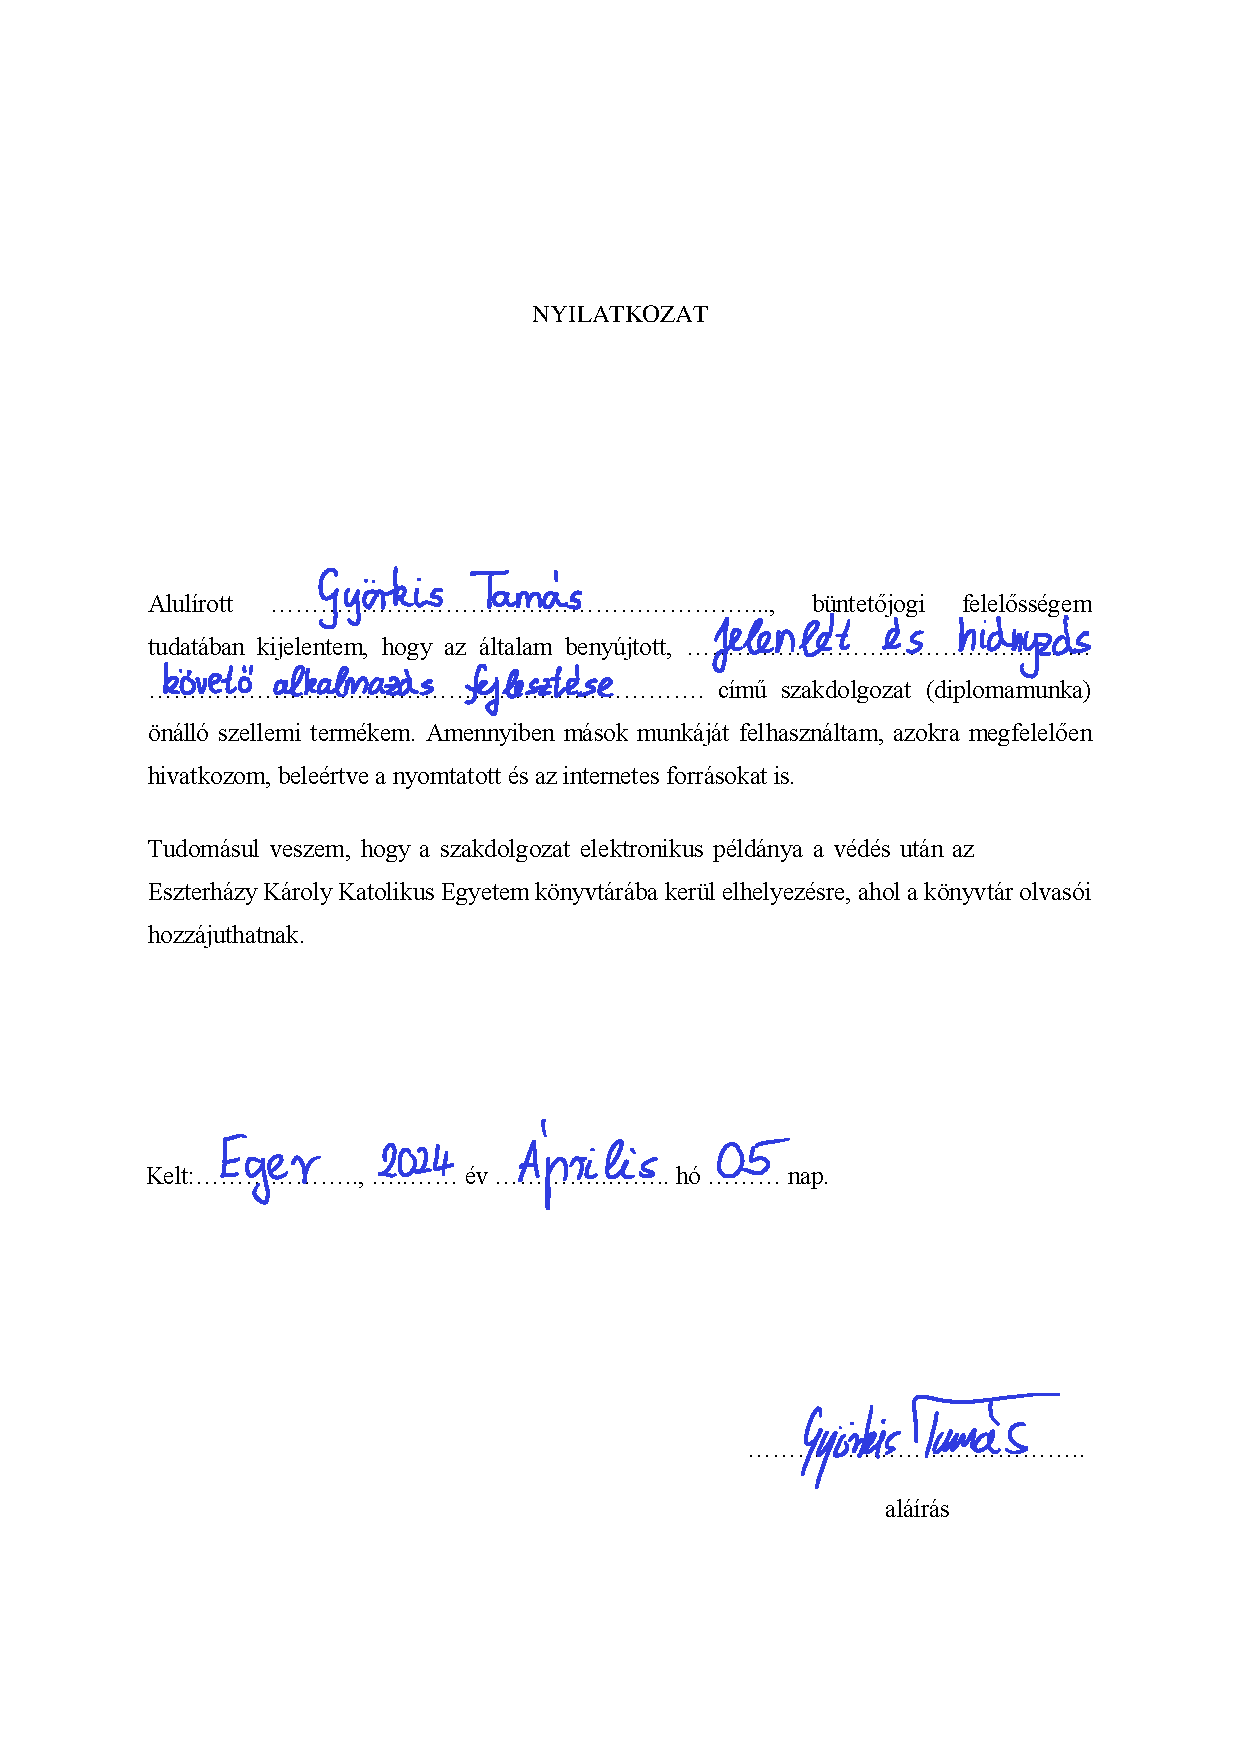
\includepdf{nyilatkozat.pdf}
\end{document}